\documentclass[border=4pt]{standalone}
\usepackage{tikz}
\usetikzlibrary{positioning, arrows.meta, shapes.geometric, calc, fit, backgrounds}
\usepackage{amsmath,amssymb}

\begin{document}
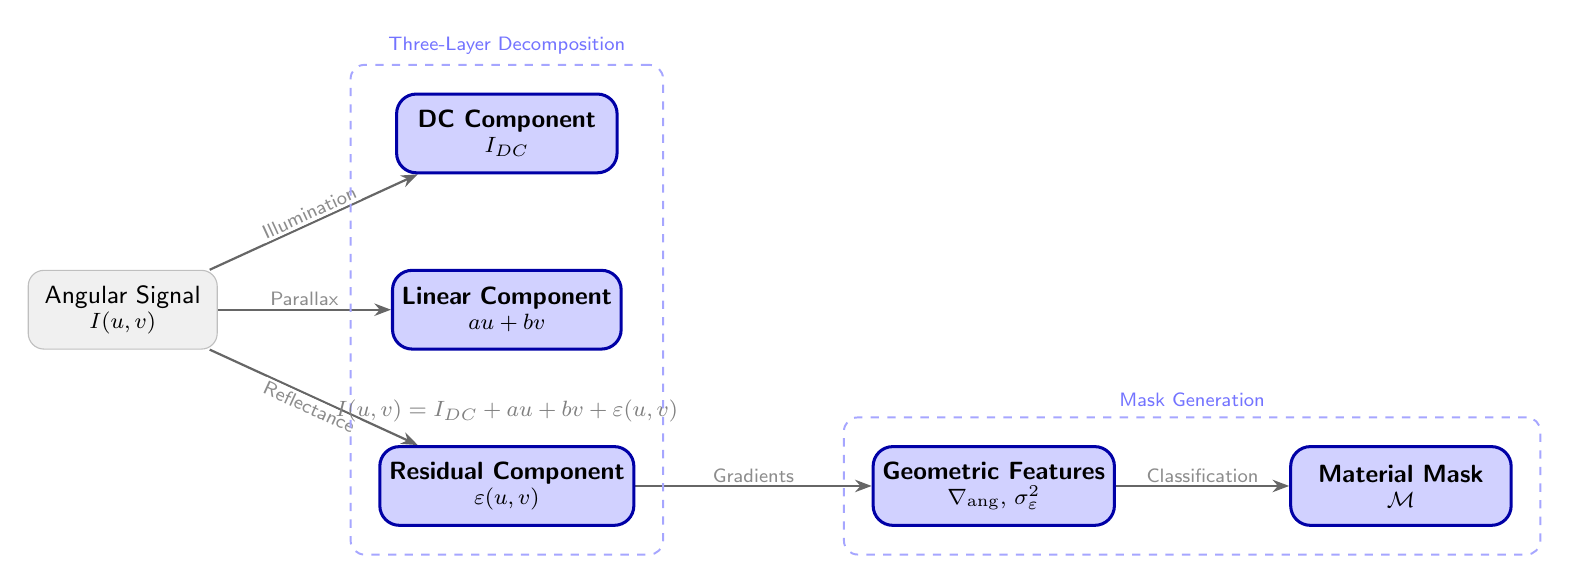
\begin{tikzpicture}[
  inputmod/.style={draw, rounded corners=2mm, minimum width=2.4cm, minimum height=1.0cm,
                fill=gray!12, draw=gray!50, align=center, font=\sffamily\small},
  innov/.style={draw, rounded corners=2.5mm, minimum width=2.8cm, minimum height=1.0cm,
                fill=blue!18, draw=blue!65!black, line width=1.1pt, align=center,
                font=\sffamily\small\bfseries},
  arr/.style={-{Stealth[length=6pt]}, thick, color=black!60},
  lbl/.style={font=\sffamily\scriptsize, text=black!45, fill=white, inner sep=1pt},
  gbox/.style={draw=blue!35, dashed, rounded corners=5pt, inner sep=10pt, line width=0.7pt},
]

% Input
\node[inputmod] (m1) {Angular Signal\\[-2pt]{\footnotesize $I(u,v)$}};

% Decomposition — m3 at same level as m1
\node[innov, right=2.2cm of m1] (m3) {Linear Component\\[-2pt]{\footnotesize $au + bv$}};
\node[innov, above=1.2cm of m3] (m2) {DC Component\\[-2pt]{\footnotesize $I_{DC}$}};
\node[innov, below=1.2cm of m3] (m4) {Residual Component\\[-2pt]{\footnotesize $\varepsilon(u,v)$}};

% Mask generation
\node[innov, right=3.0cm of m4] (m5) {Geometric Features\\[-2pt]{\footnotesize $\nabla_{\mathrm{ang}},\, \sigma^2_\varepsilon$}};
\node[innov, right=2.2cm of m5] (m6) {Material Mask\\[-2pt]{\footnotesize $\mathcal{M}$}};

% Formula annotation
\node[below=0.5cm of m3, font=\footnotesize, text=black!50] (formula)
  {$I(u,v) = I_{DC} + au + bv + \varepsilon(u,v)$};

% Arrows (on background layer)
\begin{pgfonlayer}{background}
  \draw[arr] (m1) -- node[lbl, above, sloped] {Illumination} (m2);
  \draw[arr] (m1) -- node[lbl, above] {Parallax} (m3);
  \draw[arr] (m1) -- node[lbl, below, sloped] {Reflectance} (m4);
  \draw[arr] (m4) -- node[lbl, above] {Gradients} (m5);
  \draw[arr] (m5) -- node[lbl, above] {Classification} (m6);
\end{pgfonlayer}

% Group boxes
\begin{scope}[on background layer]
  \node[gbox, fit=(m2)(m3)(m4),
        label={[font=\sffamily\scriptsize, text=blue!55]above:Three-Layer Decomposition}] (g1) {};
  \node[gbox, fit=(m5)(m6),
        label={[font=\sffamily\scriptsize, text=blue!55]above:Mask Generation}] (g2) {};
\end{scope}

\end{tikzpicture}
\end{document}